\documentclass[12pt]{article}
\usepackage[latin1]{inputenc}
\usepackage{fancyhdr}
\usepackage{geometry}
\usepackage{makeidx}
\usepackage{graphicx}
\usepackage{epigraph}

\geometry{left=2.5cm,right=2.5cm,top=2.5cm,bottom=3cm}


\title{%
		\begin{Huge}Progetto di Web Information Management\end{Huge} \\
		\begin{Large}
		Analisi di usabilit\'a di un sito
		\end{Large}
}
\date{\vspace{-2ex}}
%\author{Cristian Pirlog}

% Turn on the style
\pagestyle{fancyplain}

% Clear the header and footer
\fancyhead{}
\fancyfoot{}

% Set the footer
\fancyfoot[L]{Cristian Pirlog}
\fancyfoot[R]{\thepage}


% All the text
\begin{document}
\maketitle
\vspace{40ex}

\noindent Sito: \texttt{https://www.goodreads.com}\\

\noindent Author: \textit{Cristian Pirlog}\\
\noindent Matricola: \textit{1097011}\\
\noindent Periodo analisi: \textit{Maggio 2017}
\newpage

\tableofcontents
\newpage

\section{Analisi Preliminare}
Goodreads \'e il sito pi\'u grande al mondo per lettori e raccomandazioni di libri, creato dallo sviluppatore di software ed imprenditore americano Otis Chandler. Il 28 Marzo del 2013, Amazon annunci\'o di aver acquistato Goodreads per 150 Milioni di dollari. \\
Il sito permette agli utenti di cercare gratuitamente all' interno del database di Goodreads libri, recensioni e note. Gli utenti possono registrarsi e aggiungere a loro volta libri per generare cataloghi di librerie e liste di lettura. Inoltre, possono anche creare propri gruppi di suggerimenti di lettura, sondaggi, blog e discussioni. \\
Add oggi Goodreads conta pi\'u di 55 milioni di iscritti e oltre 1.5 Miliardi di libri aggiunti.

\subsection{Struttura}
Goodreads \'e uno social network strutturato in modo tale da permettere a chiunque di vedere i libri contenuti negli scaffali degli amici e le recensioni che questi ultimi hanno lasciato sulla loro bacheca.\\
\\Il sito dispone di un men\'u a sinistra con diverse voci \textbf{(Figure 1)}, tra le quali \textbf{Browser} e \textbf{Community}.
\begin{itemize}
\item Selezionando il primo, si ha accesso ad una lista di categorie che permettono di \textit{trovare raccomandazioni per i prossimi libri da leggere, libri premiati, giveaways, nuovi rilasci oppure semplicemente esplorare l'enorme database a disposizione}.
\item Selezionando invece Community si ha la possibilit\'a di accedere a diverse features presenti nel sito, quali\textit{ i gruppi, le discussioni, i quiz o gli eventi.} E' inoltre possibile \textit{fare delle domande agli autori pi\'u in voga del momento}.
\end{itemize}
Da questo men\'u si ha anche la possibilit\'a di accedere alla propria libreria, selezionando \textbf{My Books}. Qui si potranno anche vedere i diversi scaffali personalmente creati e riempiti. \\ \\
In alto a destra invece c'\'e un men\'u dove si pu\'o selezionare tra diverse opzioni quali notifiche, discussioni all'interno dei gruppi, messaggi, amici o informazioni del proprio profilo.
\begin{figure}
	\centering 
	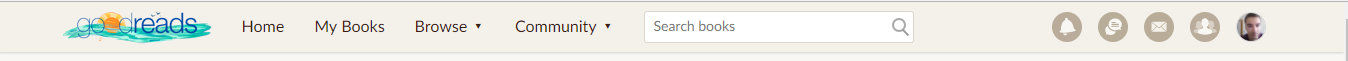
\includegraphics[width=16.5cm]{resources/headerbar.png}
	\caption{\textbf{La foto dell'header una volta loggati.}}
\end{figure}
Al centro dell'header invece, troviamo una barra di ricerca, il cui funzionamento approfondiremo pi\'u avanti.
\newpage

\begin{figure}
\section{Homepage: Le 6 W}
\begin{flushleft}
Al primissimo accesso su Goodreads quello che si visualizzer\'a sar\'a ci\'o che verr\'a rappresentato dalla figura seguente: 
\end{flushleft}
	\centering 
	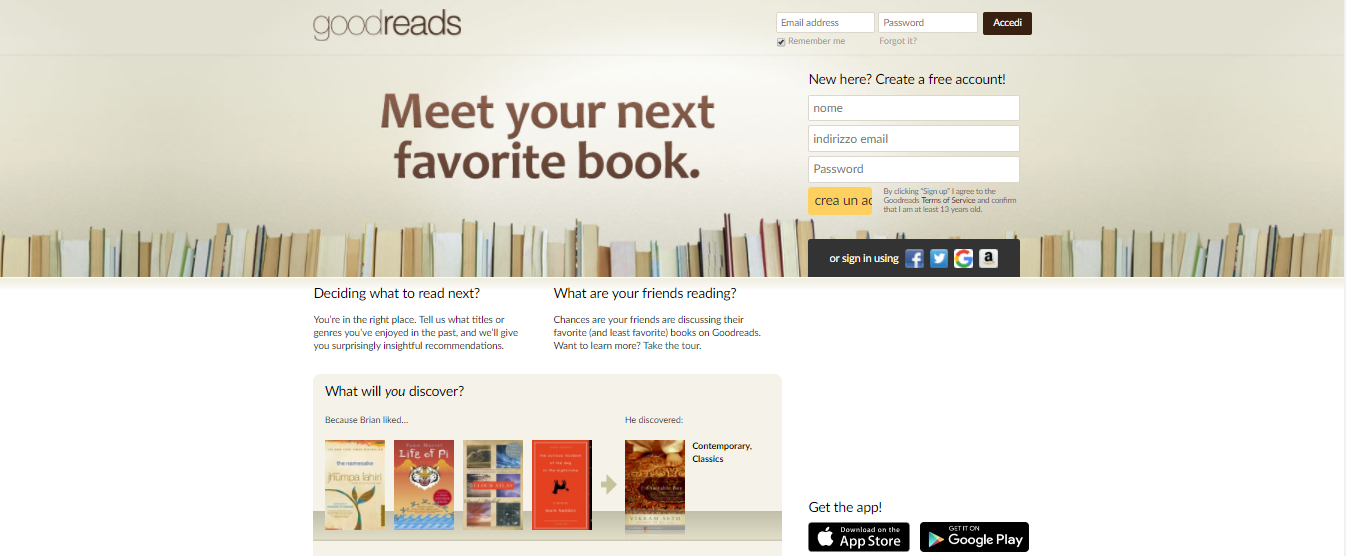
\includegraphics[width=16.5cm]{resources/homenotlogged_1.png}
	\caption{\textbf{Parte superiore della Homepage per un utente non registrato.}}
\end{figure}

\begin{flushleft}
Come si pu\'o notare dalla foto, si ha la possibilit\'a di fare diverse scelte:
\begin{enumerate}
	\item Registrarsi velocemente inserendo poche informazioni oppure collegando il proprio account di Facebook o Twitter, Google, Amazon. Questa molteplicit\'a di scelte spinge l'utente a registrarsi senza preoccuparsi di perdere troppo tempo nel compilare decine di campi. \\
	Un problema invece ben visibile \'e dato dalla localizzazione del sito in italiano. Nello specifico, il pulsante che dovrebbe servire per fare la Submit del form di registrazione contiene il testo 'crea un account' che per\'o non \'e mostrato interamente, date le ridotte dimensioni del pulsante. Un'altra pecca che si pu\'o notare \'e la capitalizzazione delle lettere dei placeholder all'interno dei tag di input e del pulsante sopra citato, la quale sembra essere stata fatta senza un criterio preciso.

	\item Loggarsi inserendo la propria e-mail e password ed avere pieno accesso al contenuto del sito.
	
	\item Informarsi sul contenuto del sito grazie ad una frase ad effetto (\textbf{Meet your next favorite book.}) che fa capire immediatamente all'utente cosa riuscir\'a a trovare, in questo caso il suo prossimo libro preferito.\\
	Ci sono inoltre anche altre informazioni che aiutano l'utente estraneo al sito a capire cosa potr\'a trovare al suo interno come ad esempio i due paragrafi titolati \textbf{Deciding what to read next?} e \textbf{What are your friends reading?}. \textbf{(Figure 2)}
	
	\item Scorrere la pagina per conoscere altre informazioni riguardo al sito. \textbf{(Figure 3)}
	
	\item Nella seconda parte della Homepage \textbf{(Figure3)}, si potranno cercare informazioni all'interno del database di Goodreads anche se non si \'e  loggati.
\end{enumerate}

\end{flushleft}

\begin{figure}
	\centering 
	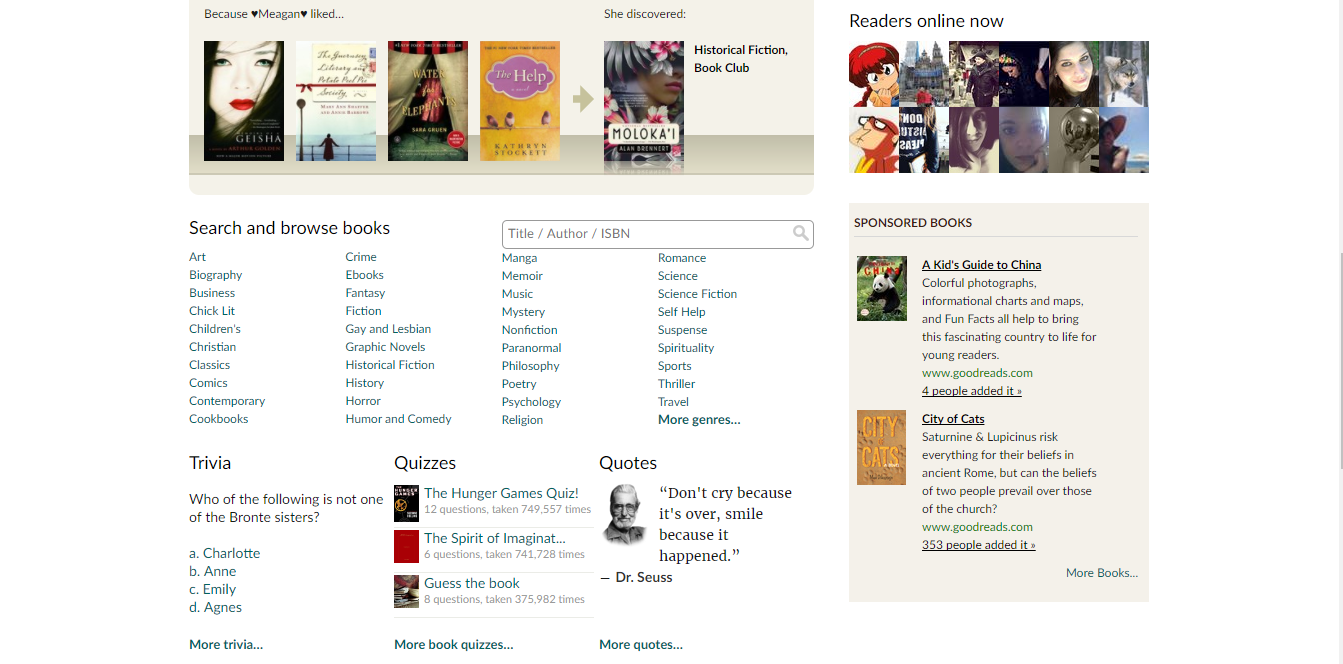
\includegraphics[width=16.5cm]{resources/homenotlogged_2.png}
	\caption{\textbf{Parte centrale della Homepage per un utente non loggato.}}
\end{figure}

\noindent {\large \textit{Dato che la gran parte delle funzionalit\'a del sito possono essere sfruttate solo se si \'e loggati, da ora in poi tratteremo solo questa sezione del sito.}}

\subsection{Where?}
\begin{center}
{\large \textit{"A che tipo di sito sono arrivato? Quale contenuto mi offre?"}}
\end{center}
\begin{figure}
	\centering 
	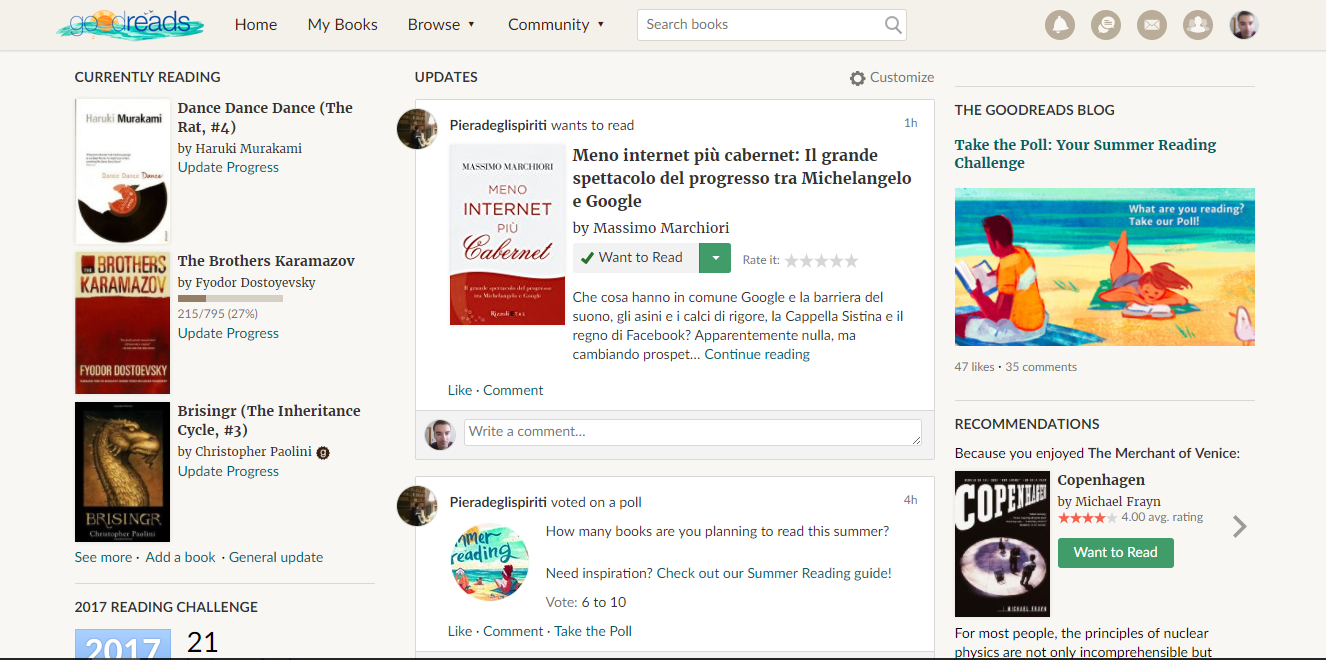
\includegraphics[width=16.5cm]{resources/homelogged_1.png}
	\caption{\textbf{Parte centrale della Homepage per un utente che si \'e appena loggato.}}
\end{figure}

\noindent Dando uno primo sguardo alla pagina principale riusciamo ad intuire immediatamente che il contenuto del sito sia composto da libri. Il nome \textit{"Goodreads"} da una mano all'utente a capire cosa effettivamente esso contenga. Il nome di un sito internet incide mediamente tra il 10\% ed il 20\% nella sua usabilit\'a e qualit\'a e Goodreads lo fa egregiamente.
Qualsiasi dubbio sul contenuto viene comunque sventato grazie ad una lettura veloce della Homepage (anche da non loggato).

\subsection{Who?}
\begin{center}
{\large \textit{"Chi rappresenta il sito?"}}
\end{center}

\noindent Goodreads rappresenta il punto di riferimento per eccellenza per gli amanti di libri. Coloro che non lo conoscono e ne vorrebbero sapere di pi\'u si troveranno davanti a 2 possibilit\'a:

\begin{enumerate}
	\item Gli utenti possono visualizzare il logo in alto a sinistra \textbf{(Figure 4)}. Clickandoci sopra l'utente verr\'a reindirizzato alla pagina \textbf{Goodreads Blog}, dove pu\'o essere letto il post pi\'u recente del sito. \\
	Nella colonna di sinistra ci sono diverse voci che permettono di informarsi ulteriormente su ci\'o che Goodreads \'e. Tra le diverse pagine si pu\'o accedere alla pagina \textbf{about us} dove si possono visualizzare i numeri del sito, il suo rank e la storia di come questo progetto ha preso vita.
	
	\item In qualsiasi momento, scrollando la pagina verso il basso gli utenti possono trovare all'interno del footer un link alla pagina \textbf{about us} precedentemente descritta.

\end{enumerate}

\noindent Per rispondere alla domanda in modo accurato, l'utente si trova quindi a dover scrollare la pagina, ma in media solo il 23\% degli utenti effettua una navigazione di questo tipo,oppure ad accedere ad una pagina differente dalla homepage. Questo comporta sicuramente un tempo pi\'u lungo in termini di permanenza nel sito. 



\subsection{Why?}
\begin{center}
{\large \textit{"Perch\'e mai dovrei fermarmi su questo sito? Quali benifici mi porta?"}}
\end{center}

Nella homepage del sito se non si \'e loggati si ha la possibilit\'a di sapere nello specifico cosa il sito offre. Goodreads aiuter\'a l'utente a trovare il prossimo libro da leggere in base alle sue preferenze oppure spulciando gli scaffali dei propri amici. Per fare tutto questo per\'o c'\'e bisono di una registrazione.\\
Se si \'e quindi registrati e loggati, nella homepage \textbf{(Figure 4)} abbiamo accesso ai pi\'u recenti aggiornamenti dei nostri amici nel corpo principale del sito. Nella barra laterale di destra possiamo vedere un'anteprima del post pi\'u recente del blog e le raccomandazioni che Goodreads offre al lettore. A sinistra invece possiamo aggiornare l'avanzamento nella lettura dei nostri libri oppure aggiungerne altri ai nostri scaffali.\\

\noindent Tutto ci\'o permette di avere una Homepage ricca di contenuti riuscendo cos\'i nell'intento di soddisfare l'utenza grazie ad un'accesso rapido a quasi tutte le funzionalit\'a principali del sito.


\subsection{What?}
\begin{center}
{\large \textit{"Cosa offre il sito?"}}
\end{center}

\noindent Un utente appena registrato potrebbe trovarsi abbastanza spaesato dato che una volta acceduti alla homepage il contenuto sar\'a pressoch\'e nullo. Tutto questo \'e compensato dal fatto che prima di registrarsi il sito presenta in modo pi\'u che soddisfacente ci\'o che l'utente trover\'a al suo interno. Inoltre dato che la maggior parte degli utenti che si registrer\'a risulter\'a effettivamente interessato al contenuto del sito, una prima ricerca approfondita tramite la barra di ricerca porter\'a l'utente ad esplorare il cuore pulsante di Goodreads.


\subsection{When?}
\begin{center}
{\large \textit{"Quali sono le ultime novit\'a presenti nel sito?"}}
\end{center}
La homepage risponde molto bene a questa domanda dato che nella colonna di destra \'e raffigurata un'anteprima del post pi\'u recente presente sul sito. Cliccandoci sopra verr\'a mostrata la pagina contenente l'intero post e i relativi commenti degli utenti.\\
Attraverso il men\'u presente all'interno dell'header possiamo anche accedere attraverso l'opzione \textbf{Browser} alla pagina \textbf{New releases}. Quest'ultima permette di accedere ad una lista che mostra gli ultimi libri usciti nel mese corrennte, mettendo l'utente davanti a tre scelte \textbf{(Figure 5)}:

\begin{figure}
	\centering 
	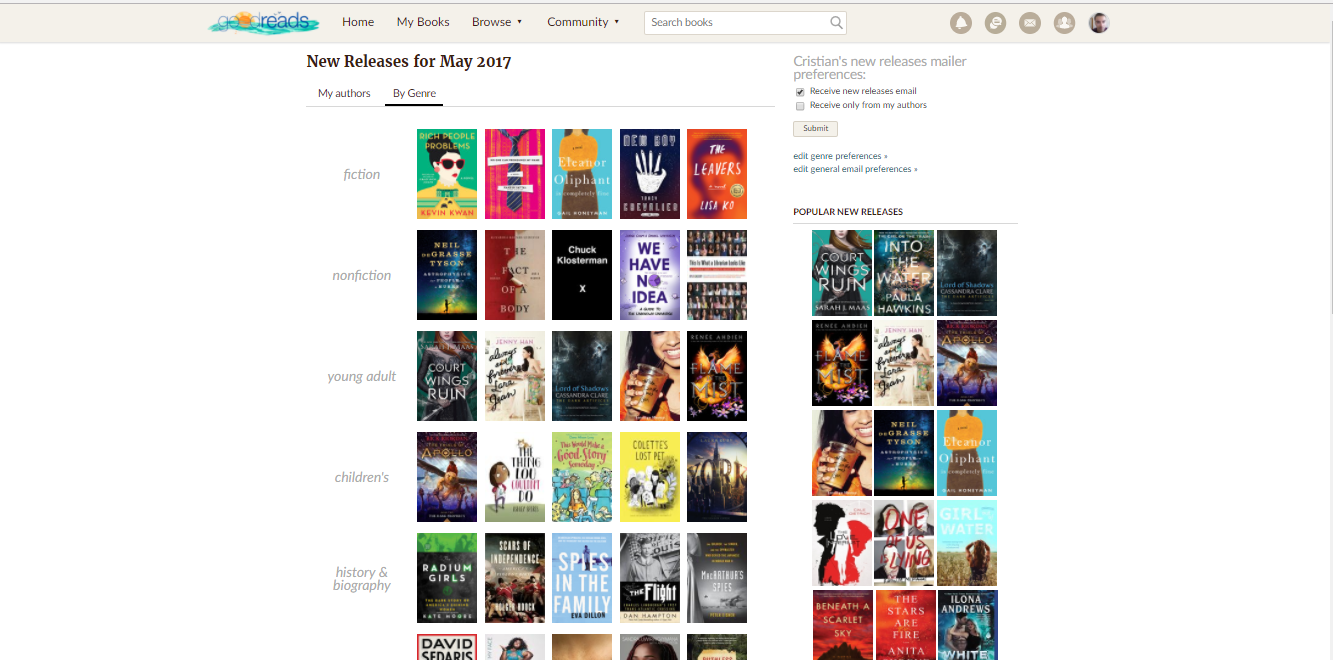
\includegraphics[width=16.5cm]{resources/newproducts.png}
	\caption{\textbf{Nuovi release di libri nel mese corrente.}}
\end{figure}

\begin{enumerate}

\item Vedere i libri che usciranno scritti dagli autori di cui si ha gi\'a letto un libro.
\item Vedere una lista di libri suddivisi per genere.
\item Vedere le uscite pi\'u popolari nella barra di destra.
\end{enumerate}

\noindent Interessante anche notare come Goodreads permetta anche di sottoscriversi ad un mailer che spedir\'a nella casella di posta dell'utente in base alle sue preferenze le nuove uscite.

\subsection{How?}
\begin{center}
{\large \textit{"In che modo si arriva alle sezioni principali del sito?"}}
\end{center}

\noindent Il men\'u nella parte alta ha un layout orizzontale a schede, e ogni scheda rappresenta una sezione diversa che potr\'a essere raggiunta all'interno del sito. Per accedere alla homepage dell'utente si pu\'o premere su \textbf{Home} ed in alternativa se si vuole raggiungere la propria lista di libri si deve premere su \textbf{My Books}. Ci sono anche altre 2 schede che permettono di accedere alle altre funzionalit\'a del sito. La prima, \textbf{Browse} che permette, come gi\'a spiegato in precedenza di raggiungere le nuove uscite, le raccomandazioni, etc. La seconda, \textbf{Community} che invece permette di accedere alla parte pi\'u social del sito, quali \textit{i Gruppi}, \textit{le Discussioni}, \textit{i Quiz} o \textit{gli Eventi}. Inoltre a sinistra, come gi\'a discusso in precedenza si pu\o' aver accesso alle informazioni personali dell'utente quali messaggi, notifiche e impostazioni dell'account.

La ricerca nella barra situata in alto \'e facilitata in modo tale da mostrare le corrispondenti scelte a seconda delle lettere che si digitano da tastiera (ricerca dinamica), ci\'o permette di sentirsi indirizzati verso la pagina desiderata. Il design del tool di ricerca \'e intuitivo e si avvicina di molto agli standard dei motori di ricerca conosciuti. Una volta che si ha scritto qualcosa, si pu\'o quindi decidere di andare alla scheda del libro interessato oppure, cliccando sulla lente accedere alla pagina che mostrer\'a i risultati della ricerca. Qui si potr\'a inoltre approfondire la ricerca attraverso diverse opzioni quali la ricerca \textit{per titolo, per autore o per genere}. \\

All'interno del sito non sono presenti problemi \textbf{gambling} dato che l'utente sapr\'a gi\'a che una volta cliccato sul link di un libro egli verr\'a trasportato alla pagina descrittiva dello stesso.\\

Per raggiungere il blog del sito, baster\'a invece cliccare sul logo oppure sulla preview a destra che riassume tramite un'immagine il contenuto dell'ultimo post.


\section{Pagine Interne}

\subsection{Pagina Interna: Choice Awards}
\begin{figure}
	\centering 
	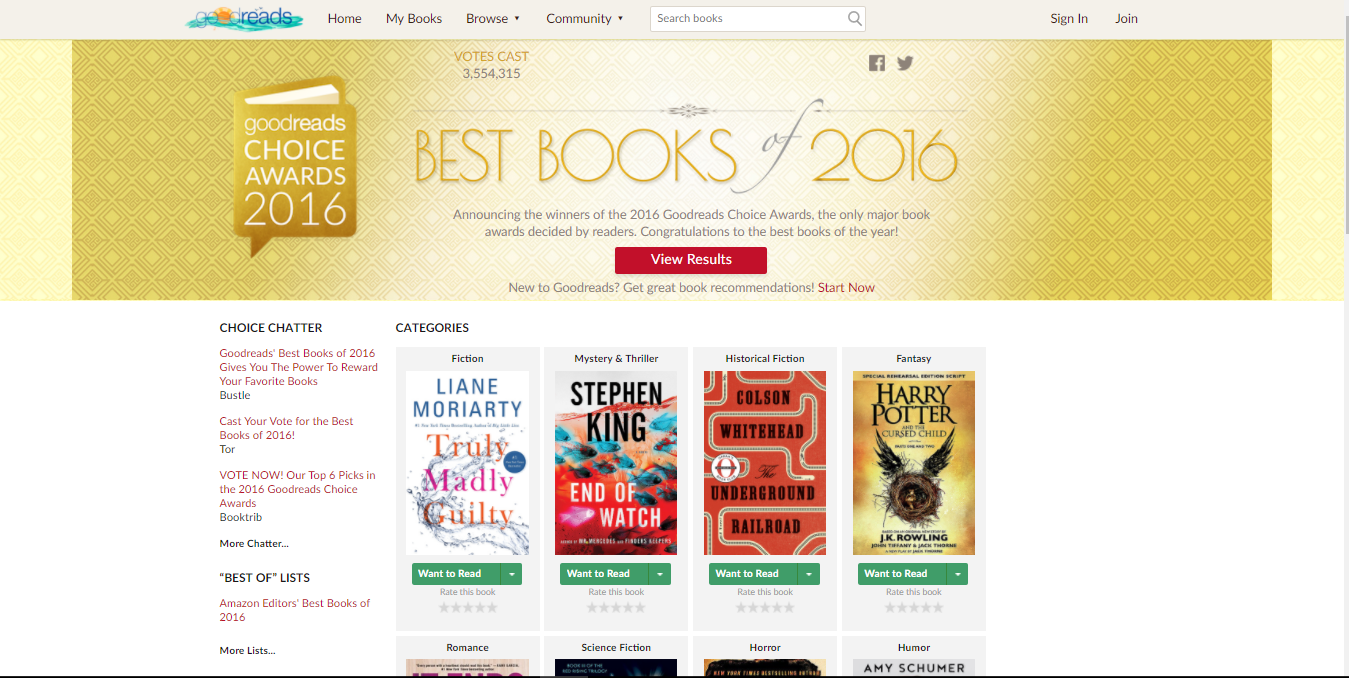
\includegraphics[width=16.5cm]{resources/choiceawards.png}
	\caption{\textbf{Pagina interna delle choice awards dove gli utenti possono vedere i migliori libri scelti dagli utenti stessi.}}
\end{figure}

A causa del fenomeno di \textit{Deep Linking} ("collegamento in profondit\'a") ogni pagina interna dovrebbe rispettare gli assi fondamentali per non generare un senso di smarrimento all'utente visitatore che \'e arrivato direttamente nella sezione interna senza passare per la homepage, una pagina quindi deve essere una "piccola homepage". Prendiamo ad esempio una pagina interna, selezionando dal men\'u la voce \textbf{Browse -$>$ Choice Awards} \textbf{(Figure 6)}. Gli assi da rispettare diventano di due tipi:

\begin{enumerate}

\item {\large \textbf{Assi opzionali:}}
	\begin{itemize}
		\item \textbf{Why:} Breve descrizione dei benefici del sito\\ 
		All'interno di questa pagina possiamo vedere come siano ancora messi in evidenza i benefici di questo sito. Dalla \textbf{Figure 6} possiamo notare come si possa aggiungere ad un personale scaffale specifico uno dei libri vincitori per ogni categoria oppure dare un voto ad uno dei libri.
		\item \textbf{When:} a che tipo di sito sono arrivato, il contenuto\\
		Questa pagina mette in mostra le copertine di alcuni libri che hanno vinto il Choice Awards. Il contenuto rimane quindi molto chiaro.
		\item \textbf{How:} indica come arrivare alle sezioni principali del sito\\
		Anche qui \'e ancora presente il men\'u in alto che aiuta l'utente a raggiungere le parti importanti del sito.		
		
	\end{itemize}		

\item {\large \textbf{Assi obbligatori:}}
	\begin{itemize}
		\item \textbf{Who:} indica chi rappresenta il sito\\
		In alto a sinistra \'e ancora presente il logo raffigurante il nome del sito e nella parte inferiore della pagina, all'interno del footer \'e presente un link alla pagina \textbf{"About us"}. Risulta quindi chiaro che cosa il sito rappresenti.
		\item \textbf{What:} cosa offre il sito\\
		Come gi\'a spiegato sopra, risulta molto intuibile immaginare che cosa il sito offra.
		\item \textbf{Where:} indica a che tipo di sito siamo arrivati\\
		Risulta molto chiaro in quale sito siamo arrivati grazie a diversi fattori: il nome del sito raffigurato all'interno del logo. Il titolo \textbf{"Best books of 2016"} e il sottotitolo che fanno intuire facilmente che si tratta di un sito rivolto agli amanti dei libri. Con ancor pi\'u enfasi si pu\'o notare la cosa grazie agli svariati libri mostrati nel corpo centrale della pagina.\\
		Potrebbe risultare discutibile la scelta di non utilizzare un breadcrumb, dato che potrebbe portare ad un problema di \textbf{"Lost in navigation"} (l'utente si trova smarrito). In compenso per\'o, come gi\'a spiegato in precedenza, il men\'u presente in alto all'interno dell'header e la barra di ricerca aiutano l'utente a viaggiare all'interno delle altre pagine senza particolari difficolt\'a. Sarebbe comunque stato molto pi\'u apprezzabile avere un breadcrumb che facesse intuire la posizione esatta all'interno del sito.
	\end{itemize}	

\end{enumerate}


\subsection{Pagina Specifica: Book}

\section{Considerazioni generali}

\section{Conclusione}

\section{Lista delle figure}
\end{document}
